%\documentstyle[astro,psfig]{article}
\documentclass{article}
\usepackage{psfig}
\usepackage{astro}
\usepackage{times}
\GoodMargins
\newcommand{\note}[1]{({\bf #1})}
\newcommand\pr{\em}                   % font for program names
\newcommand\ff{\bf}                   % font for file names
\newcommand\cc{\tt}                   % font for program code
\newcommand\ty{\sc}                   % font for file types

\title{Variability Pipeline}
\author{Eugene Magnier}

\begin{document}
\maketitle

\section{Overview}

Ptolemy is a collection of programs which act together to provide
automated reduction of images, including photometry and astrometry,
data validation, and incorporation of the resulting measurements in a
photometry database organized by star position on the sky.  Ptolemy
was designed to deal with images produced by LONEOS, the Lowell
Observatory Near Earth Object Search, to study the data stream with
astronomical goals in mind beyond just the Near-Earth Objects.  The
document deals with both the generalities of Ptolemy and also the
specifics of the LONEOS implementation.  Why Ptolemy?  Two reasons:
First, Ptolemy, the Roman Astronomery (AD 100-170) was the the first
to make a systematic map of the entire sky visible from Greece, much
like LONEOS is doing.  Second, Ptolemy I (367-283 BC), as the founder
of the Library of Alexandria, represents the ideals of collection and
organization of large quantities of knowledge).

Fig.~\ref{pipeline} shows a schematic of the {\pr Ptolemy} program
organzation.  Images to be analysed may be provided to Ptolemy either
from the telescope or from a tape archive.  Images are first analyzed
by {\pr dophot}, which produces instrumental photometry and pixel
coordinate positions for stars and other objects in the images,
writing files with a particular format, called {\ty obj} files in this
discussion.  The results from {\pr dophot} are cleaned up by a program
called {\pr fstat} which merges the header information from the image
with the most relevant parts of the {\ty obj} file, creating a new
file with the {\ty cmp} format.  Astrometry is performed on the {\ty
cmp} file with the program {\pr gastro}.  The program {\pr gastro}
makes a comparison with an astrometric reference database and only
changes {\ty cmp} header keywords as a result.  Finally, the processed
image {\ty cmp} file is added to the photometry database with the
program {\pr addstar}.  The photometry database is maintained in a
large number of files ({\ty cpt} files), each representing a small
region of sky.  There is no relationship between the image locations
and the boundaries of {\ty cpt} file.  All of the preceeding processes
occur on individual images, and would typically be performed while the
observations are occuring, or during the day following, but may be
performed at any time to add new or archived data to the database.

\begin{figure}
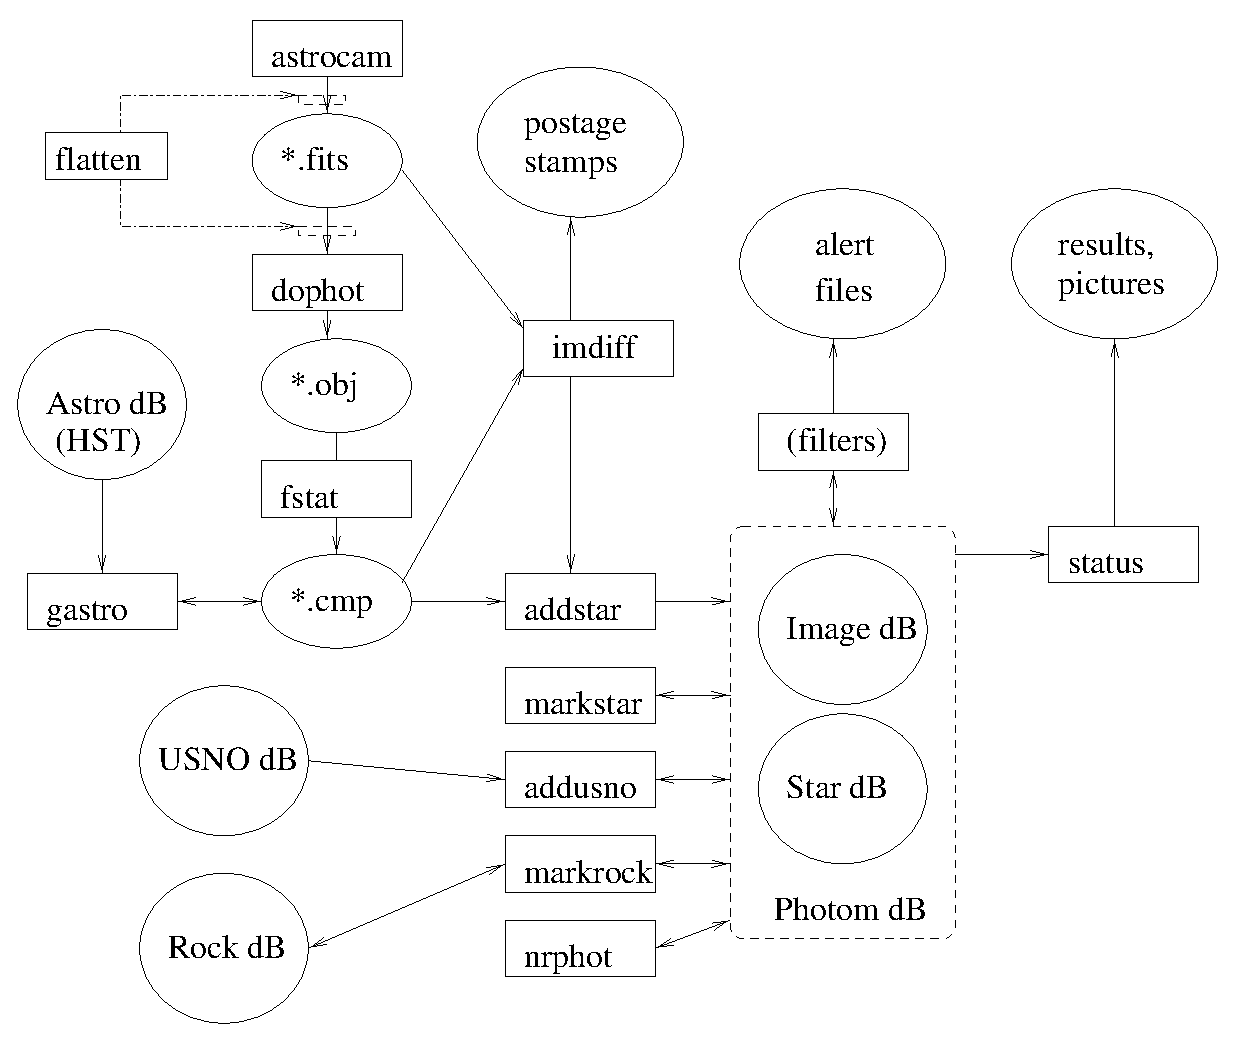
\psfig{file=schematic.eps,width=9cm}
\caption{\label{pipeline} \small
  Schematic of the photometry pipeline.  Rectangles represent
  programs, while ovals represent data products.  Arrows show the
  direction of travel of information.  The flatten routine is a filter
  whose position may change as the pipeline matures.  }
\end{figure}

Once large batches of images have been processed, a series of programs
should be run to clean up the photometry database.  First, {\pr
markstar} identifies bad data (the trails of satelites, the bleeding
columns from stars, ghost images), and flags these data points
appropriately.  Second, {\pr addusno} matches the catalog stars with
stars from the USNO database and adds the USNO magnitudes to the
photometry database.  Next, {\pr markrock} searches for likely
asteroids in the {\ty cpt} file, marks them, and writes the asteroid
observations to an asteroid database.  It also notes measurements
which are likely to be noise and cosmic rays.  Finally, {\pr nrphot}
determines relative photometric calibrations for observations in a set
of {\ty cpt} files.

\section{Image Analysis Pipeline}
\label{parallel}

\subsection{Configuration and Generalization}
With the exception of {\pr dophot}, all of the Ptolemy programs refer
to a single configuration file to determine the large number of
parameters necessary in the process.  The default parameter file is
hardwired into the programs, but an alternate configuration file may
be specified with the environment variable {\ff PIPE\_CONFIG}.  This
option makes independent processing of multiple data sources trivial.
For example, if the pipeline is to be used for both Loneos and SDSS
image analysis and display, there could be two configuration files
(eg, {\ff loneos.txt} and {\ff sdss.txt}), one for each data source.
Several important parameters would be different between these two, for
example, the initial plate scale guess for the astrometry routine, or
the parameters which define the rough chip orientation.  This scheme
allows for analysis of different types of images, with a common
destination photometry database, or for independent photometry
databases.

Data from different sources can be processed by the pipeline and
stored in the same photometry database, since all photometry is tagged
with a source ID in the database (as are the images in the image
database).  This allows us to include, for example, the USNO catalog
magnitude measurements (or a subset) in the photometry database for a
quick comparion.  Different sources may be considered different
filters, so color-color and color-magnitude diagrams could be
extracted by specifying choices for source catalog.  Currently each
object has a single primary photometric system, and individual
observations may be combined to determine that average (eg, if they
are different photometry sources with roughly the filter bandpass) or
they may be ignored when calculating relative magnitudes (eg, the USNO
magnitudes would be ignored).  This may be expanded upon by defining
multiple average magnitudes and allowing different measurements to
contribute only to the appropriate average.  The determination of the
photometry code for a particular image is currently not well defined.
There are several points in the analysis where the user (or the
controlling program) may specify the photometry source.  A table
should be kept in the photometry catalog to define the various
photometry codes.  

file names: Notice that we use a consistent naming convention through
the pipeline reductions.  The image is called {\tt foo.fits}, while
the resulting dophot-produced photometry list is called {\tt foo.obj}.

\subsection{Time representations in Ptolemy}

Every measurement in the Ptolemy database has a time stamp associated
with it, as do all of the images.  Throughout the software, the time
is represented consistently using the standard UNIX representation of
time, which consists of an unsigned integer representing the number of
seconds since 1970 Jan 01, midnight.  The time used roughly represents
UT time, though there is some subtlety here.  In reality, the time
reported at LONEOS is reported by a GPS clock, and therefore uses the
GPS zero point.  There are small, well defined differences between UT,
GPS, and WHAT IS THE THIRD ONE?  GPS - UT is a constant NN seconds,
while UT - OTHER is a function of time, as leap seconds are
accumulated in one and not the other.  While the programs all refer to
this seconds representation of GPS time, the user of the programs
usually has a few more choices.  In {\pr status}, all(?) functions
which require a time argument expect to see one of three formats. If
there is a number of the form NNNNNNNNNs, this is assumed to be the
UNIX seconds form.  If there is a number of the form NNNNNNj, this is
assumed to be a Julian date.  If there is a number of the form
YY:MM:DD,hh:mm:ss, this is assumed to be a UT date string.  Note that
the difference is in the presence of either 's', 'j', or something
else at the end of the string.  In the case of a date, it is
acceptable for the separators to be any non-numerical character, and
there may even be a trailing separator, as long as it is neither 's'
nor 'j'.  Command arguments which expect a time range may provide one
of the following units: 's' (seconds), 'm' (minutes), 'h' (hours), 'd'
(days).  Also, it is only necessary to provide as many significant
places in the date as desired.  So, if you are interested in the
images taken on UT 1999 March 03, you could run {\pr images -im
99:03:03 1d}.  

The validity range of the UNIX seconds representation of time is 143
years, so this measurement representation will become ambiguous in the
year 2113.  Note that the Y2K problem is dealt in the date string by
assuming any date with year smaller that 70 means 21st century, and
others are 19th century.  Of course, the user may explicitly type the
full 4 digit year to ensure an unambiguous answer.  Finally, the user
may refer to the current time as NOW and the current date as TODAY.

\subsection{Flat Fielding -- Mana / Flatten}

Flat fielding is performed on each image with {\pr mana} (see {\pr
mana} user's guide) using a script which interacts with the Ptolemy
controlling software.  The script is contained within a file, {\ff
flatten.pro}, in the references directory.  The script is invoked by
calling it on the command line when {\pr mana} is started.  If {\pr
mana} is started with a file name on the command line, that file is
loaded with in 'input'.  The file defines a macro '{\pr flatten}', and
also loads the flat-field file.  The flattening process is actually
done by calling within {\pr mana} the macro {\pr flatten}, with the
input and output file names as arguments.  By loading the flat-field
at the start of {\pr mana}, instead of on each execution of {\pr
flatten}, we save the load time of each flat-field image (which is 2x
the size of the basic image, being 4byte floats per pixel).  \note{The
location of the flat field is currently hard-wired in the {\pr
flatten} script - this should probably be changed in the future.}  The
macro loads a flatfield with a specific name and location, which is
actually a link; The higher-level controlling process ({\pr stage1})
creates a link to the correct flatfield.  This allows the analysis
process to use different flatfields for different situations.  At
LONEOS, we currently use a flat field generated from a well-understood
night.  This is probably not the best solution as the flatfield
changes with time.  As discussed below, the photometry solution
program, nrphot, fits a high-order polynomial to the relative
photometry, allowing for differences from the correct flatfield.
 
\subsection{Photometry -- Dophot}

Photometry is performed using a varient of {\pr dophot}, based on {\pr
Dophot 2.0} and adapted to streamline processing of many files.  With
this version of {\pr dophot}, any FITS format data is safely read in.
Instead of using staticly defined memory blocks for the images, the
necessary memory is allocated dynamically.  The image is also
converted to REAL*32 from the given BITPIX for processing.  Finally,
only a single, complete parameter file is loaded by dophot.  There is
no option for a modified and a default parameter file.  The parameter
file to be used is given, along with the input image and the output
object list on the command line when the program is run: {\cc dophot
image.fits image.obj parameter\_file}. To achive these changes, the
code from {\pr dophot} was wrapped within a C program which interprets
the command line arguments, allocates the necessary memory, and reads
in the image.  The rest of the processing is performed by {\pr dophot} in
the standard manner.  

\subsection{Cleanup -- fstat}

After an image is processed by {\pr dophot}, the object file ({\ff
foo.obj}) is converted to a more-compact, more-complete file called a
{\ty cmp} file, with a name of the form ({\ff foo.cmp}).  This
conversion is done with the program {\pr fstat}.  The {\ty cmp} file
consists of the FITS header from the original image ({\ff foo.fits}),
with some additional keywords to be used at later stages in the
analysis, followed by an ASCII list of the interesting data from ({\ff
foo.obj}).  In this list, types 6 and 8 are excluded, and only the
following values are kept:
\begin{verbatim}
X       Y     Mag   dMag t log(sky) 
1342.0  106.1 14.166 000 4 3.2
\end{verbatim}
Objects with a signal-to-noise ratio lower than a specified cutoff
({\cc MIN\_SN\_FSTAT}) are also excluded.  Some general information
about the image is derived by {\pr fstat} (FWHM, saturation and
completeness limits, number of each dophot type) and stored as
keywords in the header.  The photometry source must be specified at
this stage as one of the command line arguments, though the value used
may be overridden in one of the stages belowe.  The resulting file can
now stand on its own without reference to the original image.  The
keywords used by {\pr fstat} include the minimum signal to noise, a
rough guess at the zero point ({\cc ZERO\_PT}), and four numbers
defining the format of the {\pr dophot} {\ty obj} file.

\subsection{Astrometry -- gastro}

Astrometry is performed automatically by the program {\pr gastro}.
{\pr gastro} loads a {\ty cmp} file and determines an initial guess
for the center coordinates (based on the RA and DEC header keywords).
The program also uses the configuration information about the plate
scale and rough orientation of the image to get close to the final
solution.  Also, the true sky position of the telescope pole may be
defined to allow astrometry on images taken close to the pole.  The
comparison is made with the astrometric catalog, which may be the HST
Guide Star Catalog, or it may be any source if the data is placed in
the correct format.  \note{the astrometric reference catalog
is currently stored in an ASCII format with very limited efficiency.
It would be nice to make a standard format that has a bit of meta-data
documentation and probably a binary format to save space.}

\section{The Photometry Database}

\subsection{Photometry File Format}
The photometry database consists of a large number of photometry files
representing sections of the sky and a file containing information on
the images incorporated in the database.  These files are called
alternatively ``region files'' or {\ty cpt} files (because they have
the extension {\cc .cpt}).  The photometry files are sorted by
Declination into different directories, each consisting of a band
7.5\degree\ wide.  These directories have names like n0730,
representing the band starting at a Declination of +07:30.  The image
database ({\ff Images.dat}) is stored in the upper level directory of
this directory tree.  In fact, the locations of the {\ff Images.dat}
file, the photometry database, and such are all flexible and may be
changed by altering the configuration file.  

At LONEOS, the database is stored mostly on a RAID disk on {\ff hebe}
and a RAID disk mounted on {\ff metis}.  It is easy to split the
database across multiple file systems by using links.  Within the
database directory, there are directories for each of 24 Declination
bands (7.5 degrees tall).  The easiest way of splitting up the data is
to move some of these subdirectories to another device and creating
links to them at the appropriate place.  This is currently done by
having a directory{\ff /metis/d27/database} with the remote
directories.

The name and location of each sky region comes from the Hubble Space
Telescope Guide Star Catalog.  There is a file, {\ff GSCregions.tbl},
which can be used to find the region file appropriate for any location
on the sky.  A number of routines exist to make such a query.

Each photometry file in the photometry database contains all
observations and all average values for all stars observed within the
appropriate region on the sky.  The identity of stars is essentially
determined by their RA and DEC coordinates.  In very crowded regions,
the end user may need to double check that a neighboring star is not
contaminating individual detections (see the discusion on {\pr
addstar} below).

The photometry files are stored in a binary format, both to reduce the
volume and to speed access.  As a result, the interpretation of the
data is machine dependent: little endian machines need to swap the
data intelligently.  Fortunately, this operation is taken care of
appropriately, if the programs are compiled with the BYTESWAP option
set as needed, which is automatically set by the Makefile in the case
of a Linux machine.  For reference, Suns, SGI, and HP are all big
endian, while PCs and DECs are little endian.  The automatic
conversion takes place by using the funcions {\tt Fread} and {\tt Fwrite}
to substitute for the standard C library {\tt fread} and {\tt fwrite}
functions.  {\tt Fread} and {\tt Fwrite} are told the datatype being read,
and they know the layout of the bytes for a particular datatype.
Anytime the definitions of the relevant structures (see below) are
changed, {\tt Fread} and {\tt Fwrite} must be updated.  Fortunately, there
is only one file ({\tt Fread.c}), and it has a single byteswapping
section, making it easy to adjust the code appropriately.

The format of a single photometry database file consists four
sections:  
\begin{itemize}
\item {\bf header} -- this is a standard FITS header with room for comments
  about the file or whatever.  Since the rest of the file is not a
  standard FITS file, the SIMPLE keyword is set to False.  The three
  necessary keywords are NSTARS, NMEAS, and NMISS, which define the
  sizes of the next three sections.
\item {\bf average} -- this section contains all average measurement
  quantities for each star in the file.  There are NSTARS entries, and
  each entry is the data from a structure of type Average (defined in
  loneos.h, and discussed in more detail below).  Thus, the total size
  in bytes of this section can be found by NSTARS*sizeof(Average).
\item {\bf measure} -- this section contains the individual
  measurements for each star in the database.  There are NMEAS
  entries, and like the average section, each entry is a single
  structure, in this case of type Measure (in loneos.h, see below).
  All measurements of a single star are consecutive.  The number of
  measurements for a single star is defined by average.Nm and the
  starting entry for a single star is given by average.offset.
  Therefore, the first measurement of a specific star average[500]
  would be given by measure[average[500].offset], while the second is 
  measure[average[500].offset + 1], and so forth.  
\item {\bf missing} -- this section contains references to all missing
  measurements of a star.  This means all of those occasions when an
  image enclosed the location of a star in the database, but no star
  was detected on the image.  Similar to the case of the measure
  section, each star has a number of missing entries (which may be 0)
  given by average.Nn, and the first missing entry is given by
  average.missing.  Each missing entry value is again a structure of
  type Missing.  Currently, the only data in the structure is the time
  of the observation, which allows for an unambiguous recovery of the
  image where the star was missed.
\end{itemize}

\subsubsection*{Average Structure defined in loneos.h}
\begin{verbatim}
typedef struct {
  float R;                    /* RA  in decimal degrees */
  float D;                    /* DEC in decimal degrees */
  short int M;                /* thousandths of mag (-32.000 to 32.000 valid range) */
  unsigned short int Nm, Nn;  /* number of measurements, missing */
  short int Xp;               /* scatter in 1/100 arcsec (-327.67 to +327.67 valid range) */
  short int Xm;               /* 1000*log(chisq) for magnitude measurement */
  unsigned short int code;    /* an ID code (ie, star, ghost, satelite, etc) */
  signed int offset;          /* offset to first measurement */
  signed int missing;         /* offset to first missing obs */
} Average; /* 28 bytes / Average */
\end{verbatim}
The structure above defines the average data stored in the photometry
database for each star.  Most of the entries are self-explantory, but
some need a bit of clarification.  The entry {\tt Xm} is the magnitude
$\chi^2$ value for the star, under the assumption that the star
brightness is constant.  This $\chi^2$ incorporates the photometric
errors on each measurement and is stored as 1000 times the logarithm
of the $\chi^2$ because high dynamic range is not needed.  The entry
{\tt Xp} is the scatter about the average postion, in 10
milli-arcseconds.  As discussed above, the values of {\tt Nm} and {\tt
  Nn} give the number of measurements and missing observations for
this star, while the entries {\tt offset} and {\tt missing} point to
the first {\bf measure} and {\bf missing} entry for this star.  The
entry {\tt M} is the current best average magnitude solution for this
star (see the section on Relative Photometry).  Finally, the entry
{\tt code} is an ID code for each object, which may define a variety
of things about the object.  For example, if the object is known to be
variable, or if the object is associated with a USNO star, or if the
object is a measurement of an asteroid.  See below for details of
these definitions.

\subsubsection*{Measure Structure defined in loneos.h}
{\small
\begin{verbatim}
typedef struct {
  short int dR, dD;           /* 1/100 of arcsec (-327.67 to +327.67 valid range) */
  short int M;                /* thousandths of mag (-32.767 to 32.767 valid range) */
  short int Mcal;             /* image cal mag, thousandths of mag (-32.767 to 32.767 valid range) */
  unsigned char dM;           /* thousandths of mag (0.000 to 0.255 valid range) */
  char dophot;                /* dophot type (1-9) */
  unsigned short int source;  /* code to identify photometry source */
  unsigned int   t;           /* time in seconds (0 - 143 years valid range) */
  unsigned int average;       /* reference to corresponding average entry */
  /* upper byte of Measure.average stores flags:
   limit of 16,777,215 stars (Naverage) in a file (=0xFFFFFF) 
   flags: average & 0x1000000 */
} Measure; /* 20 bytes / Measure */
\end{verbatim}
}
The structure above defines the individual measurement data stored for
each observation of each star.  The first two entries, dR and dD, are
the difference between the average coordinates for this star and the
coordinates determined for this observation.  Clearly, if this
residual is too large, the individual measurement will not be
successfully matched with the average star position.  {\tt M} and {\tt
  dM} are the instrumental magnitude and error for this measurement,
after correction for the exposure time and a zero point (defined in
the configuration file as ZERO\_PT).  The entry {\tt t} determines the
time of the individual observation.  This is important not only for
timing purposes, but also to determine the source image for this
observation.  The time and the entry {\tt source} uniquely determine
the image in the image database that generated this measurement.
Furthermore, this correspondence allows for determination of the pixel
coordinates on the chip, by going throught the image astrometry stored
in the Image database (see below).  The entry {\tt source} is a code which
identifies the particular CCD/Telescope/Filter setup.  Each unique
{\tt source} should be treated as an independent filter set for the
purposes of accurate relative photometric comparisons.  This entry
also allows external catalog data, such as the USNO or Sloan
photometry, to be added to the database, as desired.  The entry {\tt
  average} is a pointer back to the {\bf average} section to allow
determination of the star from the measurements, in addition to the
reverse.  The bits of the upper byte of this value are reserved for
flags used to define particular situations for this measurement.
Possible values are:
\begin{itemize}
\item 1 = BLEND\_IMAGE - the star on the image matched more than one
  catalog star
\item 2 = BLEND\_CATALOG - the star in the catalog matched more than
  one image star
\item 4 = UPPER\_LIMIT - \note{not really used?}
\item 8 = CALIBRATED - relative photometry has been performed at least
  once.
\end{itemize}
The entry {\tt dophot} stores the dophot type for this particular
measurement (1-9: four extra bits in this field).   
Finally, the value {\tt Mcal} determines the photometric calibration
of this specific measurment.  This value is an offset appropriate to
this image (and if needed, this point in time and this chip position)
to bring the observations of the stars on multiple images to a common
system (see the section on relative photometry).

\subsection{Image Database}

All images for which photometry has been included in the photometry
database also have entries in an image database.  The image database
is (currently) a single file in the upper directory of the photometry
database.  The name of the file is determined by the IMAGE\_CATALOG
entry in the configuration file, and is currently set to Images.dat.
Like the photometry database files, the image database consists of a
FITS header followed by binary data.  There is only one type of binary
data: each image has an entry, which is the data from a structure of
type Image (loneos.h).  The number of images in the file is determined
by the {\tt NIMAGES} keyword.  If the number of images becomes too
large, extrapolation of the system to a set of image database files
with a reference list is quite straightforeward, and could be modeled
on the organization of the region files (eg, one image database file
for each Declination directory).

\subsubsection*{Image Structure defined in loneos.h}
{\small
\begin{verbatim}
typedef struct {
  Coords         coords;            /* 120 bytes */
  unsigned int   tzero;             /* readout time row 0 in sec (0 - 142 years valid range) */
  unsigned int   nstar;             /* number of stars on image */
  short int      secz;              /* thousanths of airmass (valid range -32.000 -- 32.000) */
  short int      NX, NY;            /* dimensions of image */
  short int      apmifit, dapmifit; /* aperture correction and error in thousandths of mag */
  short int      source;            /* identifier for CCD (each ever used will have a unique letter) */
  short int      Mcal;              /* thousandths of mag (-32.000 -- 32.000 valid range) */
  short int      dMcal;             /* thousandths of mag (-32.000 -- 32.000 valid range) */
  short int      Xm;                /* 10*log(image chi-square) */
  char           name[32];          /* name of original image */
  unsigned char  detection_limit;   /* tenths of mag (0.0 - 25.6 valid range) */
  unsigned char  saturation_limit;  /* tenths of mag (0.0 - 25.6 valid range) */
  unsigned char  cerror;            /* astrometric error: 1/50 of arcsec (0 -- 5.12 valid range) */
  unsigned char  fwhm_x, fwhm_y;    /* PSF terms in 25*arcsec (valid range 0.0 -- 10.2" ") */
  unsigned char  trate;             /* 10000 * scan rate in sec/pix (0 -- 0.0256 valid range, 
                                       typically 0.0146. this is used only to determine the time
                                       of the observation, not to find the coordinates.  1 byte
                                       gives 0.11 sec accuracy */
  float          exptime;           /* exposure time, seconds */
  char           code;              /* flag to mark an image as bad or whatever */
  char           dummy[21];         /* extra space for the future */
  short int      order;             /* number of terms used for Mrel */
  short int      Mx, My;
  short int      Mxx, Mxy, Myy;
  short int      Mxxx, Mxxy, Mxyy, Myyy;
  short int      Mxxxx, Mxxxy, Mxxyy, Mxyyy, Myyyy;
} Image;  /* 240 bytes / Image */
\end{verbatim}}

The structure above lists all of the data stored for each image.  A
substantial amount of information is stored for each image.  First,
the astrometric calibration information is stored in a {\tt Coords}
structure (see coordinate systems, above).  The upper and lower limits
of the photometry in the database (in instrumental magnitudes) is
stored in {\tt detection\_limit} and {\tt saturation\_limit}.  These
values are useful for comparison for those stars where observations
are missing.  The relationship between time and pixel coordinates is
given by {\tt tzero} and {\tt trate}.  Drift images will have a scan
rate stored in {\tt trate}, while staring images will have a value of
0.0 for this entry ({\tt tzero} then applies to the whole image).
Other important parameters are kept: the astrometric error ({\tt
  cerror}), the airmass ({\tt secz}), the exposure time ({\tt
  exptime}), the number of stars detected ({\tt nstar}), the FWHM
values ({\tt fwhm\_x, fwhm\_y}), the image name ({\tt name}), and the
size of the image ({\tt NX, NY}).  The entry {\tt source} is used as
above to define the CCD/Telescope/Filter used for this observation.
The entry {\tt code} is used to flag images in various ways.
Currently, only two bits are used, to define if the image has been
photometrically calibrated and if the calibration is acceptable.
There are 21 extra bytes are stored for future additions.

\subsection{Data Incorporation -- {\pr addstar}}

Images which are completely processed ({\pr dophot, fstat, gastro}) are
then incorporated into the photometry database with the program {\pr 
addstar}.  This program decides which region files are appropriate
for this particular image, then one-by-one adds stars from the image
to the appropriate region file.  Stars already in the catalog are
matched with stars in the new image purely by a positional comparison.
In order to avoid the difficulty of comparisons in the RA and DEC
coordinate frame, a cartesian projection is performed.  The stars from
the image being processed and the database stars in the same area are
projected onto a tangent plane and positional comparisons made in this
(locally cartesian) coordinate frame.  This avoids the dangerous
singularities at the pole and also makes the RA 0,360\degree\ boundary
a trivial problem.  

Several choices must be made in the comparison process.  If a star in
the catalog is matched with a star in the image, the new measurements
of that star are added to the database.  If a star in the database
lies in the field of the image, but is not detected, this information
is added to the list of missing data.  The only data stored in this
case is the time and source, which is sufficient to unambiguously
identify the source image from the image database.  This allows later
programs to find relevant statistics from the image database, if
necessary.  If a star is detected in the image, but is not already in
the database, a new entry is added to the database.  In addition, the
same ``missing data'' from all previous observations images which have
covered this location (ie, images already in the image database) are
included.  This last step is necessary so that the image processing
order is not important.  

Stars also run the danger of being crowded together.  Since all
comparisons are performed on the basis of position alone, crowded
fields may make for ambiguous cross-identifications.  A pair of stars
are matched if the difference in their positions is less than a
specified search radius (dependent on the scatter in the astrometric
solution for the image).  If more than one catalog stars are correlated
with a star in an image, the new measurement is added to {\em both}
catalog stars, and a flag is set noting that this observation had a
blended IMAGE.  Conversely, if a single catalog star is matched with
more than one image star, both new measurements are added to the one
catalog star, and a different flat is set, noting that this
observation had a blended CATALOG.

\section{Catalog Update and Cleaning}

Occasionally, once a large number of images have been added to the
photometry database, a set of programs should be run to clean and
update the {\ty cpt} files.  This may best be done on {\ty cpt} files after a
night's worth of data is incorporated.  These routines define bad
data, identify the USNO catalog stars, and search for asteroids and
other junk.  Most of the results from these routines are the addition
of object flags to the Average data structures (Average.code).  Most
of these routines process data within a single {\ty cpt} file at a time.

\subsection{Markstar}

The first of the update programs, {\pr markstar}, identifies bad data
and flags it.  It makes three types of identifications: bright stars,
ghost stars, and trails.  In the first case, it searches the HST guide
star catalog for bright stars within the field of the current {\ty cpt}
file.  Three types of pixels are flagged for bright stars.  Any
measurements within a circular region centered on the star are suspect
(the ``halo'' of the bright star).  Second, points along the X axis
are likely to contain flux from the diffraction spikes.  Finally,
points along the Y axis are likely to have bleeding in addition to the
diffraction spikes.  Each of these three regions has a different size
and range which must be defined in the configuration file.  The
regions are represented by a representative magnitude and a scale
parameter.  For example, the diameter $d$ of the halo for a star with
magnitude $m$ is defined as 
$d = \mbox{BRIGHT\_HALO\_SLOPE} (m - \mbox{BRIGHT\_HALO\_MAG})$.  The X and
Y axis points are defined by the length of the diffraction spike, with
an equivalent formula, and the width of the spike.  Since these are
each independent, there are 8 parameters to define the exclusion
regions of bright stars.  One of the current drawbacks of this system
is the reliance on the HST Guide Star photometry.  In the HST Guide
Star Catalog, only one photometry band is given, so no color
information is available.  The parameters currently used were defined
based on a large number of bright stars, with no adjustment for the
different effective filter system of the Loneos telescope and the HST
GSC.  Thus, occasionally very red stars will be several magnitudes
brighter in the real data than reported in the catalog.  As a result,
large numbers of bad data points in these halos and spikes may be
missed.  

The second type of bad data flagged by {\pr markstar} are the trails
from satelite and other space junk.  This portion of the program
searches for objects which land along a line and which have a high
linear density.  Parameters may be adjusted to define the width and
the necessary density or number of points in the line.  Objects in
lines are also only identified if all observations come from a common
image.  If an object only has one measurement and it is in a trail,
the entire Average is flagged to be bad.  However, if an object has
many measurements and only one is bad, the object is only flagged as
having some bad data points.  

The third type of bad data are ghost star images.  The HST GSC is
searched for stars projected across the telescope optical axis, which
is defined by the user.  All objects within a region of fixed size are
marked for ghost stars brighter than a specific cutoff magnitude.
Similar to the trails, the average is marked as bad only if all
detections of an object are ghost images.  Otherwise, it is noted that
some data may be bad.

To run 'markstar' by hand, the syntax is: {\pr markstar (file.cpt)}.
There are several optional flags, which are listed if you type
markstar by itself.

\subsection{Addusno}

The program {\pr addusno} makes two types of identifications of stars
with the USNO catalog.  First, it searches for coincidences within a
small, specified radius.  The choice of this radius is somewhat
tricky: it is important to catch the association, but also to avoid
making too many associations.  Unfortunately, astrometric errors in
the USNO catalog make it necessary to choose a surprisingly large
radius of 5\asec.  To avoid making double matches (matching the two
USNO stars to the same photometry database object), only the USNO
object closest to the object is associated.  There are also a
substantial number of stars with significant proper motion between the
USNO epochs and the current date.  It is not unusual to see 8-15\asec\ 
discrepancy for specific stars.  To catch these objects, any objects
which do not match the USNO database, but which have more than a
minimum number of measurements (2 or 3?) are searched for more distant
USNO companions.  A large, user-specified radius is used for this
search.  Of course, only USNO stars which are not already matched to
the database may be candidates for the proper motion match.  This
stage is susceptible to errors in that a slow-moving solar-system
object may be associated with a faint USNO star.  For this reason,
objects flagged as high proper motion stars should be taken with some
caution.  Of course, during the {\pr addusno} stage, no objects
already flagged as bad by {\pr markstar} will be matched with USNO
stars.  

To run 'addusno' by hand, the syntax is: {\pr addusno (file.cpt)}.
There are several optional flags, which are listed if you type
addusno by itself.

\subsection{Markrock}

Once stars have been identified with the USNO database, it is possible
to search for asteroid detections.  The program {\pr markrock}
searches within a specific {\ty cpt} file for objects which are moving along
straight lines in (X,Y,t) space.  In order for an object to be found
by {\pr markrock}, it must have three points, each with only single
measurements.  The third point must land within a specified distance
of the line projected from the first two data points.  These
comparisons are made in the three dimensional space of image position
and time.  Also, objects are only accepted if they have a speed less
than a threshold.  If an object is moving too fast, it will make a
streak on each individual image and will probably be missed anyway.
Moving objects detected in this way are flagged in the photometry
database and are also written to a Rock database.  Currently, the Rock
database just contains ASCII lists of the RA, DEC, Mag, and time for
each detection.  In fact, the data are stored in pairs of detections,
with the middle detection saved twice.  This format makes it easy to
plot lines connecting the points using the connect-the-dots plotting
style of status/kapa (see below).

One of the current drawbacks of {\pr markrock} is the insistence on
three observations with only 1 measurement each.  If an object is
moving too slowly, two of the dectections of the object may be merged
together.  Enough data is stored in the database to extract these
individual measurements, so a more sophisticated search is possible.
It is also currently the case that USNO proper motion stars are
ignored, but some of these will be asteroid detections which are
simply too close to a faint USNO stars (it has to be faint because it
would otherwise be associated with a star in the photometry
database).  

To run 'markrock' by hand, the syntax is: {\pr markrock (file.cpt)}.
There are several optional flags, which are listed if you type
markrock by itself.

\section{Relative Photometry -- nrphot}

Once the data has been incorporated in the photometry database and the
data validation routines have been run, it is possible to determine
photometric solutions for all of the images.  The program which does
this is nrphot.  It tries to find a set of solutions for each image
which reduce both the scatter per image and the scatter per star.
\note{the following section is taken from Magnier et al
1992, A\&A Supp 96, 379.  It could use a little editing to fit the
reality of the LONEOS implementation.}

In order bring the different measurements to a common photometric
system, relative photometry was performed to determine calibrations
for each image.  We used multiple measurements of individual stars on
overlapping images to connect neighboring images.  It is useful to
discuss some of the details of this process.  

A typical photometry equation can be written in a form such as:
\begin{equation}        
M_{app} = c_{\lambda} + m + a_{\lambda}*\zeta + \gamma_{\Delta\lambda}*(\Delta\lambda) \\
\label{M_mag}
\end{equation}
where $m$ is the instrumental magnitude,
\begin{equation}        
m = -2.5\log(N_{e}) + 2.5\log(t). \\
\label{inst_mag}
\end{equation}
$N_{e}$ is the number of electrons measured in a single star, $t$ is
the exposure time for the image, $M_{app}$ is the apparent magnitude
of the star in the standard system, $\zeta$ is the airmass of the
image, and $\Delta\lambda$ is the value of a color index (\ie\ $B-V$
or $V-I$) for the particular star.  The subscript $\lambda$ refers to
the filter and the subscript $\Delta\lambda$ refers to the color
index.  Notice that we are ignoring the second-order color-airmass
crossterm, and any higher order terms in $\Delta\lambda$ or $\zeta$.
In all situations, $c_{\lambda}$, $a_{\lambda}$, and
$\gamma_{\Delta\lambda}$ are calibration coefficients dependent on the
instruments and the site.  The term $c_{\lambda}$ is a factor to scale
the response of the detector.  The terms $\gamma_{\Delta\lambda}$ and
$a_{\lambda}$ give the variation of the sensitivity with the color of
the star and the airmass.  Also, Eqn. (\ref{M_mag}) is only valid for
photometric conditions.  Under non-photometric conditions, we need to
add another term to account for clouds:
\begin{equation}        
M_{app} = c_{\lambda} + m + a_{\lambda}*\zeta + \gamma_{\Delta\lambda}*(\Delta\lambda) + clouds \\
\label{M_cloud}
\end{equation}
Now, we can regroup the terms in (\ref{M_cloud}) as follows:
\begin{equation}        
m = [M_{app} - \gamma_{\Delta\lambda}*(\Delta\lambda)] - [c_{\lambda} + a_{\lambda}*\zeta + clouds]
\label{M_sep}
\end{equation}
Of the two terms on the right side of equation (\ref{M_sep}), the variables
in the first pair of brackets are dependent on the properties of the
star, those in the second pair of brackets are dependent on the image parameters,
except for $c_{\lambda}$ which is independent of both image and star.
We can now define the ``relative magnitude'' and the ``calibration
magnitude'' from (\ref{M_sep}) as follows:
\begin{eqnarray}
        m       & = & M_{rel} + M_{cal} \label{rel_phot1}\\
        M_{rel} & = & [M_{app} - \gamma_{\Delta\lambda}*(\Delta\lambda) + \Delta] \label{color}\\
        M_{cal} & = & - [c_{\lambda} + a_{\lambda}*\zeta + clouds + \Delta] \label{M_cal}
\end{eqnarray}
where $M_{rel}$ is the relative photometric magnitude of the star in
the internal system and $M_{cal}$ is a correction factor to convert
instrumental magnitudes to relative magnitudes.  The terms $\Delta$
are included in eqs. (\ref{color}) and (\ref{M_cal}) to make explicit
the fact that an arbitrary constant can be added to $M_{rel}$ and
subtracted from $M_{cal}$.  The goal of relative photometry is to
determine $M_{cal}$ for each image, then use this $M_{cal}$ to find
$M_{rel}$ for all stars from eq. (\ref{rel_phot1}).  Once one has
$M_{rel}$ for each star, one can then convert them to a standard
system ($M_{app}$) using an equation of the form of
Eqn. (\ref{color}).  In the case of the LONEOS photometry, the absence
of a filter makes an effective bandpass which is so wide that it may
be meaningless to force it to a specific, standard filter.  For the
sake of variability measurements, it is probably more sensible simply
to refer to the LONEOS system magnitudes and present a set of color
terms which give the rough relationship between stars of various
colors and the LONEOS system. 

In fact, the discussion above make a significant simplification which
assumes that all images will have a single calibration magnitude
$M_{cal}$.  In fact, it is the case in the LONEOS system that a
variety of effects introduce systematic variations across the images.
For this reason, in practice we extrapolate the above discussion to a
situation where the value of $M_{cal}$ is allowed to be a function of
position, and is fit with a 2-D polynomial of some degree.  With the
LONEOS system, we allow the fit to take polynomials of up to 4th
order, but only accept the minimum order which significantly reduces
the scatter for the particular image.

        An equation of the form (\ref{rel_phot1}) exists for each star
detected on each image.  As described, the value $m$ depends on both
the particular image and the particular star, the value of $M_{cal}$
only depends on the image, and the value of $M_{rel}$ only depends on
the particular star.  Let us label the images with the subscript $i$
and the stars with the subscript $j$.  Equation (\ref{rel_phot1}) can
then be written in the form:
\begin{equation}
m_{i,j} = M_{rel,j} + M_{cal,i} \label{rel_phot}
\end{equation}
Of course, $m_{i,j}$ only exists for certain combinations of images
and stars: not all stars appear on all images.  In the entire system
of equations, only one value of $\Delta$ (from eqs. \ref{color} and
\ref{M_cal}) can be used, but, as noted above, the {\em value}\ of
$\Delta$ is arbitrary.

        In equation (\ref{rel_phot}), both $M_{rel,j}$ and $M_{cal,i}$
are unknown quantities.  We can use a method of least squares to find
these values for the entire set of data.  We try to minimize the chi
square, defined as:
\begin{equation}
\chisq = \sum_{i,j}(m_{i,j} - M_{rel,j} - M_{cal,i})^2 / \sigma_{i,j}^2 \label{chisquare}
\end{equation}
where $\sigma_{i,j}$ is the error in the measurement $m_{i,j}$, and
the index $i$ runs over all images, while the index $j$ runs over all
stars which are multiply measured, \ie\ those stars which appear on more
than one image.

        We attempt to minimize \chisq\ analytically by finding the
derivatives of \chisq\ with respect to $M_{rel,j}$ and $M_{cal,i}$
and setting them equal to zero:
\begin{eqnarray}
\frac{\partial\chisq}{\partial M_{rel,j}} = \sum_{i}-2(m_{i,j} -
M_{rel,j} - M_{cal,i}) / \sigma_{i,j}^2 = 0  \nonumber \\
\frac{\partial\chisq}{\partial M_{cal,i}} = \sum_{j}-2(m_{i,j} -
M_{rel,j} - M_{cal,i}) / \sigma_{i,j}^2 = 0
\end{eqnarray}
In these summations, the index $i$ runs over all images in which star
$j$ appears, and the index $j$ runs over all stars which appear on
image $i$ which are multiply measured.  Solving the equality leads to
the following system of equations:
\begin{eqnarray}
R_{j}M_{rel,j} = \sum_{i}(m_{i,j} - M_{cal,i}) / \sigma_{i,j}^2 \label{system1} \\
R_{i}M_{cal,i} = \sum_{j}(m_{i,j} - M_{rel,j}) / \sigma_{i,j}^2 \label{system2}
\end{eqnarray}
where 
\begin{eqnarray}
R_{i} = \sum_{j}\frac{1}{\sigma_{i,j}^2} \nonumber \\
R_{j} = \sum_{i}\frac{1}{\sigma_{i,j}^2} 
\end{eqnarray}
Again, the index $i$ runs over all images in which star $j$ appears,
and the index $j$ runs over all stars which appear on image $i$, with
the restriction of multiple measurements.  The term $\Delta$ from
eqs. (\ref{color}) and (\ref{M_cal}) acts as an arbitrary zero point
between the relative and apparent photometric systems.

        Equations (\ref{system1}) and (\ref{system2}) are a set of
$N_{images} + N_{stars}$ linear equations with $N_{images} +
N_{stars}$ unknowns.  The unknown parameters are the terms $M_{rel,j}$
and $M_{cal,i}$.  Unfortunately, $N_{images} + N_{stars}$ is a number
on the order of 5000 - 10000, thus an analytical solution is
impractical and an iteration method must be used.  A simple iteration
method is as follows:

%\SingleSpace
\begin{enumerate}
\setlength{\parskip}{-0.05in}
\item Guess at values for each $M_{cal,i}$.
\item Use equation (\ref{system1}) to find values for $M_{rel,j}$.  
\item Substitute these $M_{rel,j}$ values into (\ref{system2}) to get a new
set of $M_{cal,i}$ values.  
\item Return to step 1.
\end{enumerate}
%\DoubleSpace
This process is repeated until some criterion is reached, such as the
\chisq\ no longer changes or reaches a desired minimum.  Although a
minimum can be found, error propagation causes severe problems
since images are only connected to neighboring images.  The end point
images are connected by \approx 50 intermediate images, and errors
propagating over such a long distance can cause severe errors.  Also,
$M_{rel,j}$ and $M_{cal,i}$ are not uniquely defined, because of the
term $\Delta$.  Therefore, during the iteration process, the values of
$M_{rel,j}$ and $M_{cal,i}$ tend to wander and do not tend to converge
($M_{cal,i}$ may be incorrect by typically 0.5 mag).  These problems
can be overcome if some of the values $M_{cal,i}$ or $M_{rel,j}$ are
known.  In this situation, the known values can be held fixed,
providing a reference point for the remaining values.  If enough
values are known across a large enough portion of the data, no image
is separated from the fixed values by many images, and errors will not
build up.

        Images taken under photometric conditions provide a set of
known $M_{cal,i}$ which can be held fixed.  This is true since, if the
image is taken under photometric conditions, the term $clouds$ in eq.
(\ref{M_cal}) is by definition 0.  The other terms in this equation
are either known ($a_{\lambda}*\zeta$) or are constant for all images
($c_{\lambda}$) and can thus be assigned to a set value, which can
later be removed with the zero point calibration.  We make an initial
assumption of the value of $a_\lambda$, but use the data themselves to
determine a best fit choice for $a_\lambda$.  The task that remains is
to determine which images were photometric.

        Since the conditions during observations varied greatly from
night to night, we decided to determine which images were photometric
from the images themselves.  To do this, we used a variation on the
iteration method described above.  Before starting the iterations, we
assume a value for $c_{\lambda}$.  We can choose this arbitrarily, and
correct for our choice in the correction to an absolute photometric
system.  Now, we perform the following iteration:

%\SingleSpace
\begin{enumerate}
\setlength{\parskip}{-0.05in}
\item Assume that all images are photometric and determine $M_{cal,i}$.
\item Find the corresponding values of $M_{rel,j}$ from equation (\ref{system1}).
\item Use these $M_{rel,j}$ values to find new values for $M_{cal,i}$.
\item Find the values of $clouds$ for each image from these $M_{cal,i}$
\item Assume that any image with a value $clouds$ more than 1 standard
deviation from the mean value (over images) has a substantial cloud
layer.  
\item Return to step 1, but use the iterated $M_{cal,i}$ values for those
images with substantial clouds.
\end{enumerate}
%\DoubleSpace
This process is continued until \chisq (eq. \ref{chisquare}) does not
change substantially.  Figure (\ref{fig:Mrel}) shows a histogram of
the occurrences of different $clouds$ values.  There are a few
important points to make about this figure.  First, there is a
concentrated peak at 0.  All of these images have essentially zero
cloud level.  As one would expect, there are a large number of images
to the right of this peak.  These are the images which were taken
through some amount of clouds.  Since the exposures were stopped if
the clouds got too thick, it is not surprising that these images taper
off at higher cloud levels.  The most curious and telling part of the
plot is the area below the 0-cloud peak.  There are many images on the
``negative cloud'' side of the peak.  Because ``negative clouds'' are
unphysical, there must be a simple explanation for this.

        We calculate the error on the relative calibration of each
image by finding the scatter of the $M_{cal,i}$ values for each image
and dividing by $\sqrt{N stars}$.  A histogram of this error for all
images is shown in Figure (\ref{fig:dMrel}).  We also show the
variation of the formal photometric error reported by \dophot\ with
magnitude for each filter in Figure (\ref{fig:dm}).  Now that we have
the values $M_{cal,i}$, we can calculate the values $M_{rel,j}$ for
every star on every image.

To run 'nrphot' by hand, the syntax is: {\pr nrphot (file.cpt)}.
There are several optional flags, which are listed if you type nrphot
by itself.  \note{discuss the optional flags in some detail}

\begin{figure}
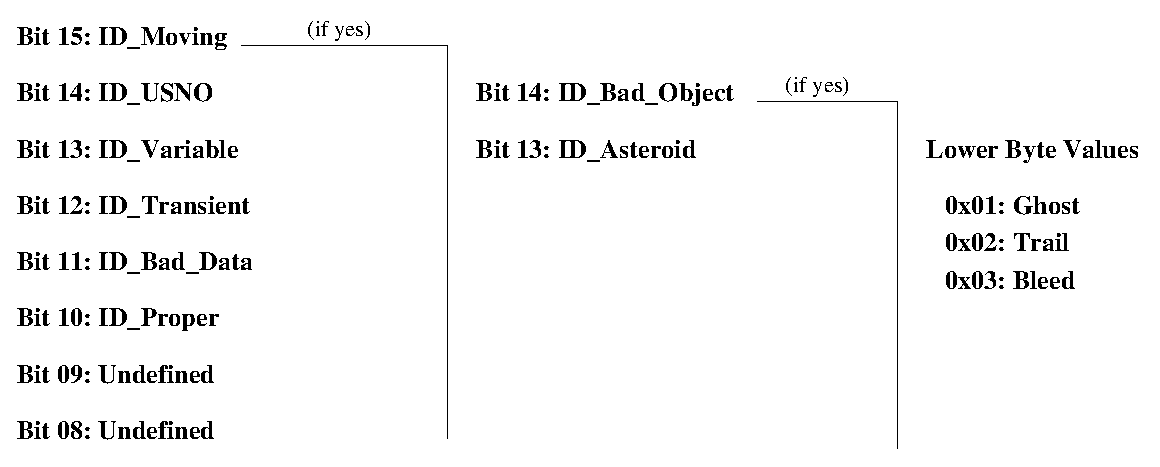
\psfig{file=flags.eps,width=9cm}
\caption{\label{flags} \small
  Pictoral representation of the Average.code flags.  The lower byte
  value is used for specific definitions of object types.  }
\end{figure}

\subsection{Data Flags}

The identifications made by the above routines are noted as a set of
flags in the Average.code structure entry.  Some of these flags are
mutually exclusive, so a certain bit may have more than one meaning,
depending on the value of other bits.  Figure~\ref{flags} shows a
pictoral representation of the meaning of the different bit fields.
The uppermost bit (bit 15) determines if the object may be considered
a ``fixed'' star or something which has no fixed location.  If it is
not fixed, and this bit is 1, then there are several options.  The
second uppermost bit (bit 14) will be set if this object is one of the
three types of bad data flagged by {\pr markstar}.  The lower byte of
code is used to define the type of bad data: ghost, trail, or bleed.
Thus, any datapoints determined to be a satelite trail will have a
code value of 0xc002 (49154 decimal).  If an object is a moving
object, but not a bad datapoint, it may be identified as a ``rock''
(an asteroid) by the program {\pr markrock}.  In this case, the flag
for an asteroid is turned on (bit 13).  Thus anything identified as a
rock by {\pr markrock} will have a code value of 0xa000.  The lower
byte of code is not yet defined for asteroids, but could be reserved
for distinguishing different classes of asteroids (ie, on the basis of
orbital speeds, and so forth).  Objects which are fixed may have a
variety of possible flags.  First, an object may be identified with a
USNO star (bit 14).  It may be found to exhibit variability (bit 13),
implying that the relative photometry routine should ignore it.  If
may be a transient object (bit 12).  Note that, while an object
associated with a USNO object may not be transient, an object which is
variable may also not be associated with a USNO object.  Thus, we need
seperate bits for variable vs transient.  Different types of variable
objects may be represented with different values of the lower byte.
For example, a Cepheid may have a specific lower byte code of 0x01,
which an RR Lyrae may have a lower byte code of 0x02.  Thus a Cepheid
associated with the USNO catalog would have a total code value of
0x6001. Finally, any of these types of non-moving objects may have
some bad individual measurements (bit 12) or may be found to have a
significant proper motion (bit 11).  It should be noted that the above
guidelines for variable stars are suggestions only, and to date (July
7, 1999), no programs currently assign or define these variability flags. 

\section{Holding it Together}

The preceeding sections describe the step-by-step analysis and
incorporation of the data from individual images.  However, the power
of the Pipeline comes in applying it to large numbers of images.  At
LONEOS, we are using four Pentinum II computers to analyse the roughly 200
images that are observed each night.  

It is best to think of the analysis of images occurring on groups of
images from a given night.  Of the set of processes discussed above,
those in section \ref{parallel} are performed on individual images
essentially independently of the other images.  The rest of the steps,
both the data incorporation ({\pr addstar}) and the database cleaning
routines occur on the entire batch, one image at a time.  Thus, the
former routines can easily be run in parallel, but the latter routines
are run in serial to avoid having two programs writing to same part of
the database at the same time.  In this model, we would process all of
the images from a night through the parallel stage of the analysis and
then run the serial stage only after the entire night is finished in
the parallel stage.  We thus have a natural division of the pipeline
into two stages.  

The implementation of the two stages involves several programs, some
of which are specific to the LONEOS situation, and others which are
more general.  There are two layers of programs which enable batch
processing of many images and repeated batch processing over many
nights.  At the highest level, are Perl scripts which choose what data
needs to be analysed and when.  These scripts tend to be more
dependent on the details of the LONEOS implementation. At the next
level down, these scripts principally call two C programs which run
the images of a given night through the pipeline.  These C programs
are more general and do not depend on the details of the LONEOS
implementation.  A defined set of files holds a log of the nights and
images that have been processed, both for the information of people
who might want to monitor the progress, but also used by the programs
to guide decisions about what to analyse next.

\subsection{Data and File Organization}

There are a set of standard locations for all of the files used and
created by Ptolemy.  These locations have both abstract names used by
the pipeline programs and specific definitions used in the LONEOS
implementation.  In general, the definitions of the files are given in
the configuration file, 'config.txt' (currently located in a
hard-wired location, but this may soon change to the mechanism used by
the lastest version of {\pr spicam} (3.0)).  The C programs all refer
to the config file for the definitions, but the Perl scripts currently
have the definitions hardwired as variable names defined in the
beginning of each file.  This should be changed to a mechanism that
looks in the config file, perhaps implemented by a standard Perl
function.

Here is a list of the main directories and their meanings:

{\bf logdir: {\ff /metis/d11/logs} - all log files and the files used
by the Perl scripts to control their actions (except locks) go here.

{\bf workspace}: {\ff /irene/d11/workspace} - the intermediate
analysis stages go here, and the tarred, gzipped directory files stay
here.

{\bf dumpspace}: {\ff /pallas/d1} - used by slurp to store images
downloaded from the tape archive.

{\bf database}: {\ff /hebe/d27/database} - the result database, and
also the locks and the {\ff Rocks.dat} file.

{\bf references}: {\ff /metis/d11/references} - a variety of reference
data, including the HST GSC, the USNO catalog, the config files, and
so forth.

{\bf source}: {\ff /metis/d11/src/ohana} - all of the programs source,
binaries, and scripts relevant to running the Pipeline are contained
in these directories.

\subsection{lastnight}

The first step in the process is the Perl script {\pr lastnight},
which is highly dependent on the specifics of the LONEOS setup.  It
looks at the disks used by the observers to write the images from a
given night.  Images are written to a directory called {\ff
/pallas/d[1-6]/YYMMDD} where {\ff YYMMDD} is an abbreviation for the
current night's date (ie, 990223).  Many files use this naming scheme,
so we will refer to such a name as {\ff YYMMDD}.  All of the images
are stored in this directory with names {\ff yyyyMMDDxxxxb.fits} where
{\ff yyyy} is the full year, {\ff MM} is month, {\ff DD} is date, and
{\ff xxxx} is a sequence number.  The 'b' refers to the 'b' CCD, and
the '.fits' extension is required.  The script {\pr lastnight} is
called by a cron job scheduled for 7am on {\ff hebe.lowell.edu} (note
that the clock on hebe is set to PST, not local MST - fix this some
day!  see also man crontab for details on setting up a cron job).  The
script searches the disks {\ff /pallas/d[1-6]} for a directory of the
right form (basically any directory beginning with a number).  By
default, the program demands that the directory have the name derived
from today's date, but with the flag {\pr -any}, it will accept any
directory.  It then checks to see if this directory has been already
been analysed (ie, it is included in the {\ff processed.log} file).
If not, it lists all files in that directory with the right ending
(\ff b.fits}) and places these names in a file, {\ff
/metis/d11/logs/YYMMDD.inlist}.  It also writes the name of the
directory (along with some other data) in a file {\ff extracted.log}.
When it has successfully ended and identified some data, it calls the
next script, {\pr stage1} and then quits.

\subsection{slurp}

An alternative to {\pr lastnight} is the Perl script {\pr slurp},
which looks for data on the tape archive.  This script looks at the
{\ff tape.log} file and compares it to the file {\ff processed.log}|.
It tries to identify nights listed in the file {\ff tape.log} which
have not been included in the {\ff processed.log}.  If it finds any,
it tries to download as much of the data as will fit on the disk {\ff
/pallas/d1}.  This script is called from within the {\pr stage1}
script and is invoked if {\pr stage1} is run without any data already
in the file {\ff extracted.log.

A related pair program are the {\pr load} \& {\pr unload} C programs
which are needed for loading and unloading the tape jukebox.  The
first is called with, {\pr load N}, which takes tape number N and
loads it into the tape drive.  The second version, called with {\pr
unload N} takes the tape and returns it to its slot.  Note that the
jukebox does not know by itself what number tape is in the drive, so
{\pr unload} needs to be told the correct one.  If it is mis-led, it
will complain and refuse to return the tape.  It is important to check
on the other users of the tape drive to be sure it is not occupied.
This is done with the {\pr llock}, {\pr lunlock} and {\pr llockstat}
programs.  The first, {\pr llock} lets you lock a particular service,
etc, while the last {\pr llockstat} lists the devices which have been
allocated.

\subsection{stage1}

The Perl script {\pr stage1} takes the image list produced by {\pr
lastnight} or {\pr slurp} ({\ff YYMMDD.inlist}) and passes the list to
the controller program {\pr control1} which performs the parallel
analysis.  The script has a few features to decide which files have
been analysed through the pipeline and to what extent.  If {\pr
stage1} is called, it should be able to figure out 1) if there is data
ready to be analysed (ie, there is a new date reference in the file
{\ff extracted.log}), 2) if the data has been partially analysed (ie,
the date reference in {\ff extracted.log} has not been put in {\ff
processed.log}, but there are entries in the file {\ff
YYMMDD.outlist}), and 3) which data needs to be run through which part
of the pipeline (ie, it decides which of the images in {\ff
YYMMDD.outlist} have succeeded at which stages of the analysis, and
starts them at the appropriate spot).  These features are most useful
if the analysis crashes in the middle or needs to be restarted.  The
{\pr stage1} script is meant to be run without any arguments and it
will figure out what needs to be done.  The only possible argument is
the -once flag.  This flag tells {\pr stage1} to analyse the data it
finds and quit when it finishes, and not call another instance of
itself.  Otherwise, when it is done, it will restart itself, and since
there is no new data in {\ff extracted.log}, it will start a {\pr
slurp} process to get data from the archive.  If there is no data in
the archive either, this process will sleep for an hour and try again.
After a few attempts (2 days?), {\pr stage1} will give up and quit
without restarting itself.  The script writes a log file called {\ff
\$scriptdir/stage1.NN.log} where NN is a number in sequence between
all runs of {\pr stage1}.  A file {\ff stage1.count} keeps track of
which number NN we are on.  When {\pr stage1} has finished the
analysis of a night's data, it writes the date in {\ff processed.log}
to let other processes know what has been analysed.  The bulk of {\pr
stage1} is not dependent on details of the LONEOS setup, but it does
expect the files to have the naming scheme described above.

\subsection{stage2}
The serial stage processes are run by the Perl scrip {\pr stage2}.
Normally, this script is always running.  It waits for the name of a
night to be added to the {\ff processed.log} file, presumably by {\pr
stage1}.  Once it finds a new name in this file, it looks for the
appropriate images in the file {\ff YYMMDD.addlist}.  It then submits
the list to the second controlling program {\pr control2}, which runs
the images through {\pr addstar}.  Images which are successfully run
through addstar have their {\ff *bf.fits} (flattened image) and {\ff
*.obj} (dophot output) files deleted.  When the entire night is done,
the rest of the {\ff *.obj} and {\ff *bf.fits} images are deleted by
{\pr stage2}, the directory with the {\ff *.cmp} and {\ff *.log} files
is tared and gzipped into the file {\ff YYMMNN.tgz}.  The directory is
then deleted.  Finally, {\pr stage2} calls the scripts {\pr
cleaning.pl} and {\pr run.phot} which runs the cleanup programs ({\pr
markstar - nrphot}) on the database.  After a successful run, {\pr
stage2} will automatically respawn a new copy that waits until more
data arrives.

\subsection{control1 / control2}
These two C-programs perform the tasks of farming the images out to
the different machines for analysis.  The two programs are essentially
identical, but {\pr control1} is allowed to use all machines and {\pr
control2} can only use one ({\ff hebe.lowell.edu}, which has the database
local to it).  These controller programs start off by executing remote
shells (using {\pr ssh}) on a set of machines.  These shells are then used
to execute the remote commands and are kept open the entire time the
process runs.  

Both control programs maintain a list of images in a set of queues.  A
set of rules defines the order in which each image travels through the
queues.  Each queue is associated with a single process (ie, {\pr
flatten}, astrometry, etc).  Images which successfully run through a
queue are sent on to the defined 'next' queue, while images which fail
are instead sent to the defined 'fail' queue.  In most cases, the
'fail' queue is a process which marks the image as bad and write the
name in a file, and then puts the image in the 'done' queue.  However,
it is possible for the 'fail' queue to be another attempt, such as in
the case of astrometry.  In this example, images which fail the
default astrometry are run through a second queue which tries again
with the {\pr -loneos} flag set (this flag makes the assumption that
the header information about the LONEOS region number for the image is
correct, not the RA/DEC information).

The {\pr ssh} connections on the remote machines are handled as child
processes with communication through the {\ff stdin} and {\ff
stdout/stderr} pipes.  Messages can be sent back and forth though
these pipes, and messages which are received from a process associated
with an image are written to a log file with the name {\ff
imagename.log} (where imagename is the root name of the image).  The
only required messages from the program are messages saying
``SUCCESS'' or ``ERROR''.  The programs therefore all end with either
of these words.  The programs are started within the controller as a
command to the shell followed by an echo of ``PROCESS DONE''.  If the
controller sees the message ``PROCESS DONE'' without either
``SUCCESS'' or ``FAILURE'' (after waiting an appropriately long time),
it assumes the program crashed.  Currently, no timeout is available
for the programs.  The flat-field process is run in {\pr mana} and is
a slightly special case.  We avoid re-loading the same flat many times
by starting a {\pr mana} process once and running the flatten
procedures as {\pr mana} function calls.  The images which are
analysed (with an indicator of success or failure at each stage) are
written to a file named {\ff YYMMDD.addlist} by the {\pr control1} and
\ff YYMMDD.outlist} by {\pr control2}.

\subsection{Lock files}

A variety of locking mechanisms are used to avoid overwriting the
database or running more than one version of the controlling programs.
There is a Perl program, {\pr locks}, which allows the user to set or
check the state of the different locks. All programs which write to
the database check for the existence of a lock on the database and
refuse to run if it exists.  The {\pr control1/2} programs and the
{\pr stage1/2} programs check for their own lock files and only run if
they don't exist.  Finally, the user can set the locks 'kill' or
'halt' for either {\pr stage1} or {\pr stage2}.  The first tells the
process to stop immediately, taking care of bookkeeping first.  The
second tells the process to finish the current set of images but not
start a new version.

\subsection{Other Perl Scripts} 

there are several other scripts which are either used to do some
simple function or may be used by the maintainer to check on the
status of the Ptolemy exectution.  The two programs {\pr checkoutlist}
and {\pr checkaddlist} take a list of {\ff YYMMDD.outlist} or {\ff
YYMMDD.addlist} files and list the number of images in the file and
the number of successes at each analysis stage.  There programs {\pr
cleaning.pl} and {\pr run.phot} deal with the cleanup programs and the
running of {\pr nrphot}.  The program {\pr backup.stuff} takes the
first 4 characters of the year/month file names and backs up to the
jukebox tape all tar files for the given month.

\section{Operational Issues and Subtleties}

The current LONEOS system runs principally on four Intel machines
under Linux.  The existing system has been generally quite stable over
the past year of operation, but there are some subtleties.  One
significant issue is the RAID disk attached to {\ff hebe.lowell.edu}.
This device is a set of three 9 GB disks merged into one 27GB RAID
disk.  The current problem with the /hebe/d27 RAID results from the
poor way it was setup.  It was set up without much knowledge of the
(at the time) rather rudimentary linux RAID system.  As a result, the
implementation is such that the disk will not automatically be
configured and mounted at boot time.  There is a script {\ff
/root/mdstart} which lists the step to setup the RAID correctly.  It
would be helpful if the {\ff rc.local} or {\ff rc.sysinit} files were
fixed to start, fsck and mount the RAID automatically at boot.  The
setup on {\ff metis} is substantially more mature and is correctly
implemented.  It comes up when the machine boots.

\section{Visualization -- Status}

Visualization of the data in the photometry database can best be
performed with the program {\pr status}.  This is a command-line
driven program with a math and macro language which makes it easy to
perform complex tasks.  

First, a few notes about the user interface.  The interface has an
interaction similar to {\pr tcsh}.  The arrows allow editing of
previous commands.  You can also use emacs-like commands such as
cntl-a to reach the beginning of the line and cntl-e to reach the end.
There is command and file completion: if you type part of a command
(as the first thing on a line) and then type tab, it will fill in as
much as possible, until the word is not unique.  Typing tab twice at
that point will list the possible endings.  For any but the first word
on a line, the same thing will happen for the files in the current
directory.  It is also possible to type just a fraction of a command,
as long as it is unique.  An ambiguous command will list the possible
alternatives.  For example:
\begin{verbatim}
status: c
ambiguous command: c ( catalog cgrid clear create cursor )
\end{verbatim}

The shell is essentially an interpretive programming language.
Variables are set as follows:
\begin{verbatim}
status: $fred = 10
\end{verbatim}
Any expression within curly brackets \{\} is assumed
to be an arithmetical expression and is evaluated before the line is
executed.  For example:
\begin{verbatim}
echo {$fred*dcos(45)}
\end{verbatim}
would give the response 7.07107.  There are math functions cos, sin,
and tan, which operate on radian expressions, and also dcos, dsin,
dtan, which operate on degree expressions.  There are also the
equivalent inverse functions: eg., asin and dasin return radians and
degrees, respectively.  The help section on Math defines all of the
available math functions.  

\subsection{Miscellaneous Commands}
\begin{verbatim}
!                         -- system call
?                         -- list commands 
??                        -- list variables 
echo                      -- type this line 
exec                      -- system call
exit                      -- exit program 
help                      -- get help on a function 
output                    -- redirect output to file
quit                      -- exit program 
scan                      -- scan line from keyboard or file to variable 
wait                      -- wait until return is typed
which                     -- show command 
\end{verbatim}
Most of these are self-explanatory.  The command ?? prints the system
variables.  The {\tt help} command will provide help on a single
command or, without any arguments, will list all available help
files (this includes general help not associated with a specific
command).  

\subsection{Shell Programing}
\begin{verbatim}
break                     -- escape from function 
for                       -- loops 
if                        -- logical cases 
input                     -- read command lines from a file 
macro                     -- deal with the macros 
\end{verbatim}

There are several options for programming in {\pr status}.  First, a
file which contains a series of commands can be executed with {\tt
  input (filename)}.  It is also possible to define macros which will
behave much like regular commands.  A macro is defined by typing {\tt
  macro name} or {\tt macro create name} followed by the commands.
Arguments to the macro are assigned to the variables \$1 .. \$N and
the number of arguments is given by \$0.  Macros may be defined in
{\tt input} files, and in fact when {\tt status} is started, it loads
the file {\tt \~/.statusrc} which may contain default macros.  Simple
loops and if statements can be performed, and are quite useful for
complex macros.  

``If'' statements are similar in syntax to C if statements, but only
the following logical operators are available: $>$, $<$, $=$, !, $|$,
and \&.  Notice that (currently) there is no $>=$ or $<=$ symbol.  The
operator ! means ``not equal to'', but cannot be used to negate a
logical value.  The operators $|$ and \& have the meaning of ``or'' and
``and'' respectively.  Math expresions in the if statement must be
contained in curly braces, as elsewhere.  Variables with string values
may use the logical $=$ operator to test if two strings are the same.
``For'' loops are quite simplistic.  The form is:
\begin{verbatim}
for var first last delta
 (commands)
end
\end{verbatim}
The value of {\tt \$var} will start at the value {\tt first} and increment by
{\tt delta} after each loop.  The loop will stop after {\tt \$var} is greater
than {\tt stop}.  The value {\tt delta} is optional, with 1 assumed.
The value of {\tt \$var} may be changed during the loop, and if set
beyong the value of {\tt last} will end the loop early.  

\subsection{Vector Plotting}

\begin{verbatim}
box                       -- draw a box on the plot
clear                     -- erase plot
create                    -- create a new vector
cursor                    -- get coords from cursor
grid                      -- plot cartesian grid
hist                      -- create histogram from a vector
labels                    -- define labels for plot
limits                    -- define plot limits
plot                      -- plot a pair of vectors
print                     -- write vectors to file
ps                        -- define labels for plot
set                       -- vector math
style                     -- set the style for graph plots
vectors                   -- list vectors
zplot                     -- plot scaled points 
\end{verbatim}

In addition to scalar variables, {\tt status} can manipulate and
display 1-D vector variables.  Many of the commands which extract data
from the photometry database place the data in vectors as well as
plotting them.  A vector can also be created based on a number
sequence with the command {\tt create name Nelements start delta}.
The resulting vector has $Nelements$ entries, starting at a value of
$start$ and running until $start + delta*Nelements$.  If $delta$ is
0.0, all elements will have the value of $start$.  A histogram of a vector
may be made with the command {\tt hist}, which creates a new vector
containing the histogram of the first vector.  The data range and bin
size of the histogram are defined in same way as with create.  This
makes it easy to create the index vector that goes with a histogram
vector:  
\begin{verbatim}
hist y Ny 1 100 0.1
create dx 1 100 0.1
\end{verbatim}
The above will create a histogram of y in Ny and the index in dx.
Plotting this with {\tt plot dx Ny} will show the histogram.

Vector math is performed with a command of the form {\tt set new =
  (expression)}.  The expression is some math function employing
vectors and scalars.  A complete listing of the math operators
available in {\tt set} can be found in the help for {\tt set}.

Once vectors are defined, they may be plotted.  A pair of vectors can
be plotted against each other if they have the same number of entries.
The plotting is performed on the graphics window, Kapa.  There are
actually several graphics windows available to {\tt status}, any of
which may be used to plot at any time.  Some of the more complex
operations default to either graphics window 0 or 1, depending on the
context.  Except for those functions with a pre-defined window, all
plotting functions apply to the current graphics window unless an
option {\tt -n N} is given to specify a different window.  The
plotting style is determined by the command {\tt style} which can set
the line width, the line type (solid, dashed, dotted, etc), the point
type (box, cross, etc), the point size, the color, and whether a pair
of vectors is plotted as a sequence of points, a set of connected
lines, or a histogram.  Some functions which make plots use their own
styles, as discussed below.  The function {\tt limits} lets the user
set the range of the plot axes, or check the current setting.  The
command {\tt plot} will plot a pair of vectors on the current graphics
window using the current plotting style for that window.  The command
{\tt zplot} will plot a pair of vectors with the point size scaled by
a third vector, with maximum and minimum point sizes representing
specified values.  The {\tt cursor} command goes the other way: this
command puts the Kapa window in cursor mode and waits for input from
Kapa.  The user can then type any alphanumeric key on the graphics
windows and will be told both the pointer location (in the graphics
coordinates) and will have the coordinates stored in {\tt status}
variables.  For example, by typing ``1'' in the sky display window,
the RA and DEC of the pointer are stored in the variables {\tt \$R1}
and {\tt \$D1}.  This command can be used to let the user define
locations or regions of interest on the Kapa window. (Future addition:
{\tt button}, which does the same with the mouse buttons).  

\subsection{Database Functions}

\begin{verbatim}
gcat                        -- get catalog at location
gimages                     -- get images at location
gstar                       -- get star statistics
extract                     -- extract average vectors from catalogs
mextract                    -- extract measurement vectors from catalogs
imstats                    -- plot image statistics
imextract                   -- extract image vectors from database
lcat                        -- list catalogs in display region
cmatch                      -- match two catalogs
\end{verbatim}

There are a variety of other commands which directly refer to the
photometry database.  Some of these functions extract data of various
types from the database, others perform more complex plotting
operations.  The commands listed above are those which simply extract
data from the database.  The first three list information relevant to
a specific RA, DEC location on the sky: {\tt gcat (RA) (DEC)} lists
the catalog at the specified location and places the name in the
variable {\tt \$CATNAME}, {\tt gimages (RA) (DEC)} lists all images
which overlap the specified location, {\tt gstars (RA) (DEC) (RADIUS)}
lists data about the stars within a specified radius of the specified
location (all numbers above are given in decimal degrees).  Similarly,
{\tt lcat} lists the catalogs in the region.  Imstats lists statistics
about each image

The next three commands extract a specific piece of information from
the photometry database and places it in a vector.  First, {\tt
  extract} will extract average values for each star and place it in a
vector.  Next, {\tt mextract} will extract measurement values for each
star and place it in a vector: as a result a single star may have
multiple entries in the measurement vectors.  Finally, {\tt imextract}
will extract image statistics into vectors (not yet implemented).


\begin{verbatim}
catalog                    -- plot catalog stars
cgrid                      -- plot sky coordinate grid
cplot                      -- plot vectors in sky coordinates
czplot                     -- plot scaled vectors in sky coordinates
images                     -- plot image boxes
imdense                    -- image density plot
lcurve                     -- plot lightcurve for a star
pcat                       -- plot catalog boundaries
region                     -- define sky region for plot
resid                      -- plot residuals
simage                     -- plot stars in an image
\end{verbatim}

There are two types of database plotting functions: those that display
or refer to the spatial charateristics of the data and those that
refer to other types of charatersitics, such as the time domain.  The
graphics window 0 is reserved for all plots of objects on the sky.
The command {\tt region} defines the current sky coordinates for plots
in graphic window 0.  The command {\tt pcat} plots the outline of all
photometry database files which are within the currently defined
region (and by default, only those with data).  {\tt images} plots the
outline of the images in the image database, while {\tt imdense} shows
the number of images at a location by randomly spacing dots within the
boundary of the images.  The command {\tt cgrid}
draws a grid in celestial coordinates on the for the current region.

The most complex, but also one of the most useful command is {\tt
  catalog}, which plots the positions of stars in the photometry
database (and others) on the sky.  There are many options to this
command.  One set allows the user to plot stars from the photometry
database (the default), from the HST GSC, or from an ASCII text file
with RA, DEC, and Mag in specified columns.  If the ASCII file has a
fixed number of bytes per line, the data can be more quickly loaded.
The size of the points may be scaled by the star magnitude, by the
number of observations of the star, or by the number of missing
datapoints for the star.  In addition, points may be plotted only if
they land in specified magnitude ranges, or with specified numbers of
measurements, or missed measurements.  Also, objects may be plotted
only if they have a specified Average.code, so that only asteroids or
only perfect stars may be plotted.  The plotted vectors may be saved,
if desired, and the source catalog epoch may be specified as different
from J2000 (only valid for ASCII data).

Several other commands relate to non-spatial charateristics of images
and stars.  {\tt lcurve} will plot a light curve for all stars within
some radius of a point.  {\tt resid} plots the photometry residuals
for a particular region file.  

\section{Some Examples}

\note{we need some better and more relevant examples}

\begin{figure}
\psfig{file=fullsky.ps,width=16cm}
\caption{\label{allsky} \small
  Map of the entire sky, and images added to database.  }
\end{figure}

Fig.~\ref{allsky} shows a map of the entire sky, and the location
of the images currently in the database.  This picture was made with
the following commands: (output is not shown) \\
\begin{verbatim}
status: region 0 0 90 gls
status: cgrid
status: style -lw 2 -c red 
status: images
status: ps
\end{verbatim}
In this example, on the graphics window, the image boxes are shown in
red.  The user now has the possiblitiy of using the cursor command to
narrow in on a specific region, and so forth.  

\begin{figure}
\psfig{file=polar.ps,width=16cm}
\caption{\label{polar} \small
  Map of the sky in polar project, and images added to database.  }
\end{figure}

Fig.~\ref{allsky} shows a map of the entire sky, and the location of
the images currently in the database from a polar project.  This
picture was made with the following commands: (output is not shown) \\ 
\begin{verbatim}
status: region 0 0 90 zea
status: cgrid
status: style -lw 2 -c red 
status: images
status: ps
\end{verbatim}
In this example, on the graphics window, the image boxes are shown in
red.  The user now has the possiblitiy of using the cursor command to
narrow in on a specific region, and so forth.  

\begin{figure}
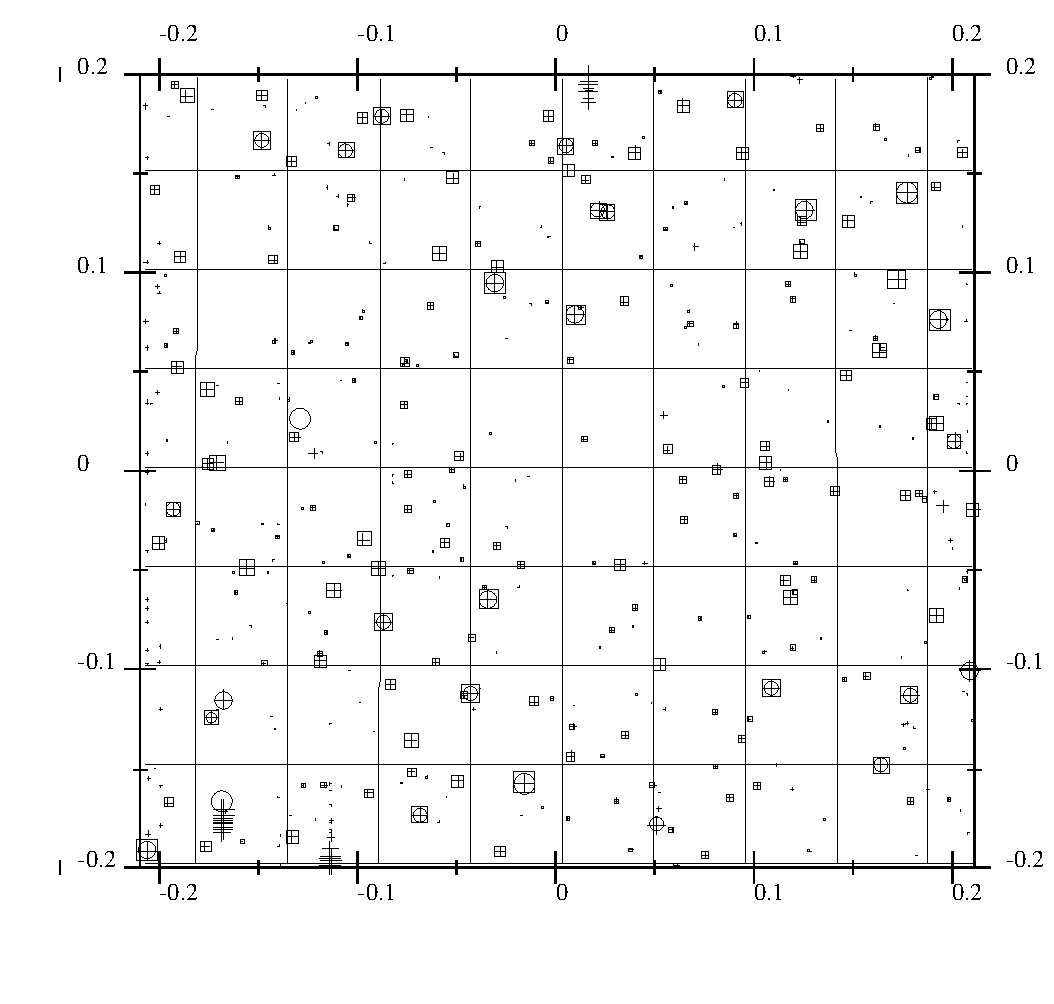
\psfig{file=catalog.ps,width=9cm}
\caption{\label{catalog} \small
  Comparison between HST GSC and photometry database astrometry.  }
\end{figure}

Fig.~\ref{catalog} shows an example comparison of the photometry
database star positions and the HST Guide Star Catalog star positions.
The crosses are all objects in the photometry database, while the
boxes are only the stars identified as USNO stars.  The circles are
the stars from the HST GSC.  The size of both points is a function of
brightness.  This plot was made with the following commands (starting
from the previous image):
\begin{verbatim}
status: cursor  (typed 1 on region of interest)
1 137.097858 22.698305
q 137.097858 22.698305
status: region $R1 $D1 0.2 TAN
status: cgrid
status: box
status: style -pt 0 
status: gcat $R1 $D1 
  0 n2230/1951.cpt *
status: style -pt 2; cat -all -m 12 18
status: style -pt 1; cat -all -m 12 18 -ID $USNO
status: style -pt 7; cat -all -m 12 18 -g
\end{verbatim}

\section{Software Distribution}

All of the code, binaries, and scripts for the Pipeline are stored in
the ohana tree at {\ff /metis/d11/src/ohana}.  The ohana directory contains
subdirs of bin, lib, include, src, config, and doc.  There is a
Makefile at the top level which calls lower-level Makefiles to build
the programs desired.  One of the important concepts in the ohana
distribution is the design of the directory layout to enable binary
support for multiple architectures.  The Makefiles use the environment
variable ARCH to determine the appropriate architecture.  The binary
and library files are stored in subdirectories of the form {\ff bin/\$ARCH}
and {\ff lib/\$ARCH}.  It is therefore necessary that users of the ohana
system architecture define the ARCH variable correctly.  It is also
necessary to include in the user's PATH the directory
{\ff /metis/d11/ohana/bin/\$ARCH}.  At LONEOS,
with the solaris sparc station and the linux machines both in use,
ARCH can take on the values of 'linux' and 'sol'.  The values 'sun4',
'irix', and 'hp' have also been used at various sites.  A simple bit
of csh script in the users .cshrc or equivalent can make this
assignment transparently:

\begin{verbatim}
set sys=`uname -s` 
switch ($sys)
 case IRIX64:
   setenv ARCH irix;
   breaksw;
 case SunOS:
   set ver=`uname -r | awk '{print substr($1,1,1)}'`;
   if ($ver == 5) then
     setenv ARCH sol
   else 
     setenv ARCH sun4
   endif
   breaksw;
 case Linux:
   setenv ARCH linux;
   breaksw;
 default:
   echo "unknown architecture";
   setenv ARCH unknown;
   breaksw;
endsw
\end{verbatim}

The Makefiles use the ARCH variable not only for destination
directories, but also for destination binary names.  All files of the
form fred.c are compiled to fred.ARCH.o (instead of fred.o), 
uninstalled libraries get the names libfred.ARCH.a (instead of
libfred.a), while uninstalled programs are called fred.ARCH.  

The perl scripts are kept in {\ff ohana/src/perl}, with links to the
appropriate bin directories.  All programs are stored in directories
of the form {\ff ohana/src/program}.  The exceptions are {\pr gastro}
(stored in {\ff ohana/src/astro}), and {\pr control1/2} (stored in
{\ff ohana/src/astro}).  Also, a variety of simple, user-level
functions are available in {\ff ohana/src/misc}.

Most of the ohana package of programs use several common libraries.
These include the {\pr readline} library (except for {\pr dophot},
this is the only part of ohana that is not written by Eugene Magnier),
which is used for command-line interface systems.  Other important
libraries are the {\pr fits} library for implementing the FITS
specifications in a convenient C-friendly environment, and the {\pr
ohana} library, consisting of basic string and other basic operations.

\section {Comparison with USNO catalog}

I have made several comparisons between the USNO catalog and results
from running images from Loneos through the photometry pipeline.  In
general, there is a good agreement between the astrometry of the two
datasets.  There are specfic areas where the two disagree, however.
First, as discussed above, the USNO star positions may be
significantly different from the observed star positions simply
because of proper motion.  The first picure in the ``Comparisons
between Loneos + USNO'' pages shows several stars with significant
proper motion.  These are currently being flagged in the photometry
database as discussed.  Other differences evident in this first
picture include the classification of bright stars and the splitting
of faint and bright stars.  In the upper right of the image, two
bright stars are visible, one of which is actually a double.  The USNO
catalog does a good job of detecting both, but it also detects and
includes as stars several diffraction spike points.  The HST GSC only
detected a single point and did not split the star at all.  The Loneos
data in our pipeline did not detect the star at all due to saturation.
A star in the upper left corner shows the ability of {\pr dophot} in
the Loneos pipeline to split double stars.  This star is, on close
inspection, clearly a double.  The USNO catalog only detects one.  The
Pipeline not only splits the two stars, but it also makes the correct
cross-identification of the stars.  

The second set of pictures shows the ability of the Loneos pipeline to
deal with small galaxies.  There are two small galaxies in this field,
both of which are broken into 4 or 5 objects by the USNO catalog, but
maintained as single objects in the Loneos pipeline.  In another
example (not shown) a bright star within the disk of a small galaxies
was clearly split from the galaxy by the pipeline (and also by USNO).

\appendix
\section{Parameter file params.txt}
\note{replace with up-to-date version from Lowell}
\begin{verbatim}
# Configuration file for Loneos analysis pipeline 

# important files and directories
IN_DIR                  /pallas
OUT_DIR                 /irene/d11/workspace
#
CATDIR                  /hebe/d27/database
IMAGE_CATALOG           /hebe/d27/database/Images.dat
IMAGE_CATALOG_TEMPLATE  /hebe/d27/database/template.cat
CATALOG_TEMPLATE        /hebe/d27/database/template.cat
ROCK_CATALOG            /hebe/d27/database/Rocks.dat
#
GSCFILE                 /metis/d11/references/GSC/GSCregions.tbl
GSC_DIR                 /metis/d11/references/GSC
USNO_CDROM              /metis/d11/references/USNO
DOPHOT_PARAMS           /metis/d11/references/config/default_parameters
FLATTEN_SCRIPT          /metis/d11/references/config/flatten.pro
LONEOS_REGIONS          /metis/d11/references/config/regions.map

# parameters for "fstat"
# instrumental mag zero point
ZERO_PT                 24.5
DOPHOT_CHAR_LINE        129
DOPHOT_TYPE_FIELD       5
DOPHOT_AP_FIELD         91
DOPHOT_PSF_FIELD        52
MIN_SN_FSTAT            6.0

# parameters for "gastro"
DEFAULT_RADIUS   32.0
MINIMUM_RADIUS   1.5
MIN_ERROR        0.6
MIN_PRECISE      0.12
CCD_PC1_1        1
CCD_PC2_2        -1    # for loneos
CCD_PC1_2        0
CCD_PC2_1        0
ASEC_PIX         2.82
NFIELD           3.0
MMIN             6.0
ROT_ZERO         0
dROT             1.0
NROT             2
POLAR_AXIS_RA    -90.0
POLAR_AXIS_DEC   89.88
RA_OFFSET        -90.0
DEC_OFFSET        0.0

# parameters for "addstar"
# airmass extinction coefficient (in mag / airmass)
NSIGMA                  3.0
ALPHA                   0.03
XOVERSCAN               60
YOVERSCAN               50

# parameters for "controller"
NEW_IMAGES              images.dat
USERNAME                gene
PASSWORD                gene

# here we list all available machines
NMACHINES               6
MACHINE0                metis
MACHINE1                hebe
MACHINE2                iris
MACHINE3                irene
#MACHINE4               juno
MACHINE4                ceres
MACHINE5                vesta

# here we define which machines which are always free
fMACHINE0               1
fMACHINE1               1
fMACHINE2               1
fMACHINE3               1
fMACHINE4               0
fMACHINE5               0
fMACHINE6               0

LOCAL_MACHINE           1  # machine with catalog on local disk

# parameters for "status"
TIME_REFERENCE          90/01/01 00:00:00

# parameters for "nrphot"
# make this one small to boost change of getting an early region 
TAU                     3.0             
SCATTER_LIM             15.0
MAG_LIM                 17.0
IMAGE_SCATTER           0.075
NIMAGE_SCATTER          1.5
STAR_SCATTER            0.05

### parameters for "markstar"
SEARCH_RADIUS           360   # region for initial trail hunt, in arcsec 
TRAIL_WIDTH             5.0   # expected trail width, in arcsec
NANGLE_BINS             180   # Number of angular bins in 180 degrees
NPTSINLINE              5     # minimum points needed for trail
MIN_DENSITY             0.025 # minimum linear density in star/arcsec
SPACE_SIGMA             10.0  # how much denser than average for trail?
# parameters defining bright star exclusion regions
BRIGHT_XTRAIL_WIDTH       5.0 # faintest sat. star
BRIGHT_XTRAIL_MAG         9.5 # faintest sat. star
BRIGHT_XTRAIL_SLOPE     -80.0 # exclusion radius = BRIGHT_SLOPE * (mag - BRIGHT_MAG)
BRIGHT_YTRAIL_WIDTH       5.0 # faintest sat. star
BRIGHT_YTRAIL_MAG        11.0 # faintest sat. star
BRIGHT_YTRAIL_SLOPE    -400.0 # exclusion radius = BRIGHT_SLOPE * (mag - BRIGHT_MAG)
BRIGHT_HALO_MAG           8.5 # faintest sat. star
BRIGHT_HALO_SLOPE       -28.0 # exclusion radius = BRIGHT_SLOPE * (mag - BRIGHT_MAG)
# parameters which define the ghosts
GHOST_MAG               7.5
GHOST_RADIUS            200   # in arcsec
OPTICAL_AXIS1           2154.0
OPTICAL_AXIS2           2193.0

# parameters for "addusno"
USNO_RADIUS             5.0   # in arcsec
USNO_PROPER             20.0   # in arcsec
USNO_RED                1000  # code for USNO Red data
USNO_BLUE               1001  # code for USNO Blue data

# parameters for "markrock"
ROCK_RADIUS             2.0   # in arcsec
ROCK_MAX_RADIUS         20.0  # in arcsec
ROCK_MAX_SPEED          0.1   # in arcsec / sec
\end{verbatim}

\section{Creating New Flats}

The LONEOS implementation of the analysis pipeline has a limited
ability to choose a flatfield image.  There is a mechanism in the
stage1 script to select a flatfield on the basis of the photcode
entry.  It works like this: there is a fixed directory for all
flatfield files, currently {\ff /metis/d11/reference}.  This directory
is written in the file {\ff flatten.pro}, and also in the script {\pr
stage1}.  Each flatfield has a name like {\ff flatcodeN.fits}, where N
is the relevant photcode.  The {\pr mana} macro '{\pr flatten}' in
{\ff flatten.pro} loads the file {\ff \$flatdir/flatfield.fits} (OR
SOMETHING LIKE THAT), which is a link to the correct flat.  The script
{\pr stage1} has the job of deciding which is the correct photcode and
setting the link appropriately.

This then begs the question of how this flatfield file should be
created and assigned a new photcode.  The flatfield is NOT made
nightly from the entire set of data, as one might expect.  This is not
done because of the problems of scattered light in the telescope.  The
widefield of the LONEOS telescope makes it somewhat succeptible to
light at relatively large incident angles.  As a result, a median
image made from images of the night sky will have different amounts of
scattered light depending on the overall sky brightness.  In our
experience, the presence of light clouds and just a small moon (as
little as a quarter) make the resulting median image a very poor
representation of the chip response.  Our solution to this problem is
to choose a good night, in which the sky is very dark, and make a
flatfield from that collection of images.  As a result, there is too
much decision-making involved to allow the pipeline to make this
decision.  Instead, we have chosen to only infrequently make a new
flat from the data, choosing those nights that we are confident will
not introduce excess scattered light.  

There are a set of scripts and programs to make the flatfield image.
The process involves first removing the bias and dark from the image,
by subtracting a dark image, then medianing the resulting images.
\note{find these scripts...}  In fact, instead of medianing,
medianfilter returns the average of the fraction of pixels with values
between f1 and f2 percent of the total range of the pixel data.

\section{Daily Monitoring of the Pipeline}

On a daily basis, the pipeline generally runs by itself without any
intervention.  There are a few checks that can be made to be sure the
process is running OK.

First, it is good to see if the disk space is sufficient.  There is a
component to stage1 which will keep it from running the analysis if
there is less space on the destination disk ({\ff /irene/d11/workspace})
than 1.1 times the amount of space in the source directory
({\ff /pallas/d?/YYMMDD}).

Second, it is a good idea to see if the nightly cron job is checking
for new data and if the data is getting analysed.  If data was created
last night, there should be a set of files in the log directory ({\ff
/metis/d11/logs}) of the form {\ff YYMMDD.inlist}, {\ff
YYMMDD.addlist}, and {\ff YYMMDD.outlist}.  If these files do not
exist, it may just mean that no data was created last night.  In that
case, the tail of the file {\ff /metis/d11/logs/lastnight} should say
something like 'there is no new data to analyse'.  \note{It would be
nice to include some notification scripts at the end of {\pr
lastnight}, {\pr stage1} and {\pr stage2} which sent some mail
describing what had been accomplished the previous night}.

If data was created, and these files exist, it is a good idea then to
check that the analysis of the images was reasonable and didn't fail
on most of the images.  There are two Perl scripts to check on this.
First, {\pr checkaddlist [filenames]} will take a list of {\ff
*.addlist} files and, for each file, list the total number of images,
then the number that failed for each of the four {\pr stage1}
processes, {\pr flatten}, {\pr dophot}, {\pr fstat}, and {\pr gastro}.
A typical run might look like this:

\begin{verbatim}
hebe: checkaddlist 9907??.addlist
990701: 206 0 0 0 0
990703: 199 5 0 0 0
990705: 150 10 1 0 1
\end{verbatim}

It is actually unusual for any except the {\pr flatten} process to
fail, and it might be typical for 1 or 2 of those to fail, since they
will represent aborted images or images which failed to write
everything to disk.  The second Perl script is {\pr checkoutlist}
which works just the same with the {\ff YYMMDD.outlist} files, but
only give statistics on the {\pr addstar} process.  Here, it is more
common for several images to fail {\pr addstar}.  At the current time,
{\pr gastro} does not always return a fail status if it finds a bogus
solution (recent work in late July may have fixed all of those fail
status messages).  Images which fail {\pr gastro} are mostly those
which were taken when the sky was too bright and all that is seen is
the sky itself, or the focus frames, or the very short images taken of
bright stars to check the coords.  If the images fail {\pr gastro} but
do not get rejected with an error status, they are rejected by {\pr
addstar} on the basis of header keywords which will say 0 stars used
astrometry.  It is also the case that {\pr gastro} should return a
failure status if the astrometric solution is sufficiently far from
Cartesian.  In general, the astrometry does not fail with a solution
close to the correct solution.  I have found several examples of
images with extremely wrong astrometric solutions, with very large
non-Cartesian images on the sky.  There are also a number of failures
near the pole with signficantly off astrometry, but close to an
accurate solution.  The should now be rejected by {\pr gastro}.

\section{Restarting the Pipeline}

It is difficult to predict the future, so it is hard to give guidance
on solving future problems.  Some of the things which might happen
would include having one of the machines which serve a disk go down or
having the disks fill up.  If this happens, it is possible that the
run of a given night will have failed completely, or mostly.  There
are a variety of things to do to recover from these situations.

\subsection{Deleting data from the archive}

The program {\pr delstar} lets the user delete a set of data from the
database.  There are several options for this.  The first example is:
{\pr delstar 199902040015b.cmp}.  In this form, delstar uses the
astrometry information in the image header to find the measurements
and delete them from the database, along with the image from the image
database.  This form requires the datafile *.cmp to exist in the local
directory.  The second form, {\pr delstar 911012323 1}, uses the given
time in standard UNIX seconds form to identify the image in the image
database and delete both the image and the measurements.  \note{does
delstar expect a UNIX seconds date, or can it take any of the
variations available in 'status'?}  It is easy to associate time with
image with the status function {\pr findimages} or {\pr gimage} which
list images covering a specific location.

The third form of {\pr delstar} is used to clean up the database if an
image is deleted but not all measurements from that image are removed.
The routine {\pr addstar} uses the astrometric information for an
image and the X,Y coordinates of each object in the image to locate
the object in the database.  Several other routines do the reverse
process of finding the location of objects within the images.  The
function which performs this association needs to find all database
*.cpt files which are covered by the image.  The existing
implemenation is relatively quick, but not the most general possible.
In some rare cases, parts of an image will not be found.  This is
normally not an issue since few functions need to find all stars in a
given image from scratch.  However, if such an image is deleted, some
of the stars from that image may get left behind.  These orphaned
stars can be deleted with the command {\pr delstar region.cpt -orphan
STUFF??}.

\subsection{Deleting a night from the pipeline}

If the analysis for a specific night fails miserably, it is probably
necessary to delete the entire night and then encourage the system to
redo that night.  It is easy to delete an entire night with {\pr
delstar} by giving a time interval which includes (only) the night in
question.  It is also easy to find the value of the time in seconds
with the {\pr status} function {\pr ctimes}.  (At some point, {\pr
delstar} should incorporate the code from {\pr status} which does the
time format conversion automatically).  This process will remove the
night in question from the database.  But before the analysis can be
re-run, Ptolemy needs to forget that it already ran that night before.
Every night which has been analysed gets included in the log files
{\ff processed.log} and {\pr addstared.log}.  The appropriate entry
from these files needs to be deleted.  It is also necessary to delete
the files {\ff YYMMDD.addlist} and {\ff YYMMDD.outlist} from the log
directory.  If the {\ff extracted.log} file exists, it should be
deleted as well.  All of this is predicated on the assumption that the
user has halted all processing by Ptolemy before trying to fix
anything.  At this point, it is possible to restart the analysis.
This can be done in several possible ways.  If the night in question
has already been put on tape, it has to be extracted.  The program
{\pr slurp} will automatically find data which has not been extracted
from the tape, download it, and set up the appropriate files.
Unfortunately, {\pr slurp} uses the file {\ff tape.log} which is not
automatically generated.  It is therefore necessary to add a line to
{\ff tape.log} (in {\ff /metis/d11/logs}) for the night in question,
which should look just like the entry in the directory {\ff
pallas:/root/tape.log}.  Instead of actually running {\pr slurp},
however, the user should just run {\pr stage1 -once} which will
perform one run of {\pr stage1} and then end.  If there is no pending
data (nothing in {\ff extracted.log} that has not been analysed), then
{\pr stage1} will automatically call {\pr slurp} in the correct
fashion (ie, on {\ff pallas}), run through the analysis, and then exit
without restarting.

If the night's data has not been deleted yet, then it is not necessary
to run {\pr slurp} as the script {\pr lastnight} will do the job.  The
cronscript for {\pr lastnight} uses the -today option so that the
automatic analysis will not reattempt any nights still on pallas.
Instead, it will be necessary for the user to run {\pr lastnight
-any}, which will also take care of running {\pr stage1}. This should be
safe at anytime, as the lock functions keep multiple instances of the
programs from running, but it is better to do this with enough time to
allow the process to finish before the next night's data is ready for
processing.

If the pipeline has been interrupted, it will probably be necessary to
restart {\pr stage2} as well.  Since {\pr stage2} always restarts
itself on exit, there is no cron job for it to make the initial start.
(This probably should be introduced into the /etc/rc.local file, or
some cron implementation for {\pr stage2} worked out).  Note that both
{\pr stage1} and {\pr stage2} take no arguments except the optional
{\pr -once} flag.  They make their own decisions about the correct log
file number and so forth.

If the {\pr lastnight} cron job gets lost, there is a copy of the
necessary cron script {\ff
/metis/d11/src/ohana/src/perl/lastnight.cron}.  This can be submitted
with {\pr crontab lastnight.cron}.

\section{Data backup}

Backups are the still rather primitive in implementation for the
LONEOS system.  There are two things which should be backed up, but
only one currently has a good scheme.  The database itself does not
have a backup process at the moment.  This is a bad situation, but not
an easy one to solve.  The database is very large, over 30 GB, which
is comparable to the space on a single AIC tape.  At the moment, we
are satisfied with simply saving the intermediate results directories,
all of the {\ff YYMMDD.tgz} files.  If the entire database is
destroyed, these files can be used to rebuild the database in a
relatively short time (currently, about a week).  The script {\pr
backup.stuff} will backup a group of files.  A good method is to
backup a month at a time.  These will become a single tar file on the
AIC tape, and a month's worth of data is a reasonable amount of disk
space for future downloads.

\end{document}

At LONEOS, the images are
written to the disk from the camera by {\pr astrocam}, the camera
controller user interface.  The resulting images are FITS files (which
may be arbitrarily sized) and have header keyword parameters RA and
DEC specifying rough celestial coordinates.  